\chapter{Results and Discussion}
\label{chap:results}

In this chapter we present results from the evaluation phase. Given the iterative nature of design research, some adjustments were made between iterations. While we began looking at two different NoSQL databases and one relational database to use for implementing archive prototypes, we ended up moving forward with only Elasticsearch and TokuDB. This was due to an increased knowledge over time about the domain, archive use cases and the technologies themselves. Following the initial iterations, we came to the conclusion that Elasticsearch was the more interesting of the two NoSQL alternatives to pursue further and that doing so would yield more interesting results. Still, to have something to relate it to, the decision was made to also perform most of the evaluation points for TokuDB as well.
As such, the results included in this section focus on the last iteration of development where all focus was put on Elasticsearch and TokuDB. 

\section{Testing environment}
Access was given to a dedicated server\footnotemark\ in order to achieve more control of the environment so as to get more dependable measurements. However, it should be emphasized that the purpose of doing the measurements was not to perform an experiment and we do not claim to have done so. Instead, the goal was to assess initial feasibility of the solutions and see if they would perform in an adequate manner. More specifically, we ask if the measurements of disk usage, memory utilization, insertion time, query response time etc.\ are good enough to warrant going forward beyond prototype construction.

\footnotetext{Specs: Redhat Linux 6.6, 256GB RAM, 2TB storage}

\section{Data separation}
For evaluation and testing purposes, access was given to a CIMS instance with a database containing about 2 years' worth of data (see figure~\ref{fig:jeTrend}), where the job event table contains about 480 million rows. This is the largest database with real data that could be safely accessed for evaluation purposes, without disturbing production environments. Using the developed software components for transforming and migrating data, all relevant data from the CIMS instance was migrated to the databases of the archive prototypes. Overall the migration process worked well in terms of transforming data to fit the non-relational model and using the developed software components to perform their respective tasks.

%Some measurements were done during the migration process, specifically how much time the process took. This was done mainly to get ball park figures to answer if the expected time is likely to be hours, days or weeks.

\section{Query support}

The set of important queries defined in section~\ref{sec:usecases} has been implemented for the archive prototype using Elasticsearch. This section describes the outcome of this implementation along with reasoning about the complexity of the queries. Query support for TokuDB is not addressed since in this case, queries and schema are identical to CIMS so there is no translation needed.

The set of important queries translated based on the non-relational schema (section~\ref{nosqlmodel}) was defined previously in section~\ref{sec:archiveapi}. These queries were implemented as part of an API component than can be used for testing purposes and by other systems. Implementation of all queries was successful in the sense that the queries can certainly be expressed using the query language of Elasticsearch, if application side joins are allowed. However, the effectiveness of the queries is highly dependent on the design of the non-relational schema. Several differences in query properties of the archive prototype compared to the CIMS database has been noted, as is to be expected. Due to the denormalization of data, fewer joins are required for the non-relational databases and the joins that are performed are done on the application level. Joins on this level leads to more round trips to the database, but lightens the computational resources used by the database. As long as application side joins are simple in nature, i.e.\ fetch one record, get its id and fetch related records, we believe using application side joins are acceptable. For anything else, data should be denormalized so that joins are not needed.

%\hiddensubsection{Elasticsearch}


%\hiddensubsection{MongoDB}
%
%Vad skiljer sig mysql queriesen mot nosql:
%    * Joins görs på applikationsnivå
%    * Mer roundtrips
%    * Index på allt (es)
%    * Ad hoc queries (es)
%    * Fri text sök, could enable better data analysis (es)

%\begin{table}[h]
%\begin{tabular}{|l|l|l|}
%\hline
%\textbf{High level query}                & \textbf{Supported} & \textbf{Comment}           \\ \hline
%Get build                                    & Y                                                                                        &                            \\ \hline
%Get build information                        & Y                                                                                        &                            \\ \hline
%Get build for root test suite                & Y                                                                                        &                            \\ \hline
%Get trouble reports for build                & Y                                                                                        &                            \\ \hline
%Get trouble report fixes for build           & Y                                                                                        &                            \\ \hline
%Get trouble reports for product and revision & Y                                                                                        &                            \\ \hline
%Get test suite children                      & Y                                                                                        &                            \\ \hline
%Get test case in build                       & Y                                                                                        &                            \\ \hline
%Get test suite in build                      & Y                                                                                        &                            \\ \hline
%Get root test suite for test case/test suite & Y                                                                                        &                            \\ \hline
%Get test case by name                        & Y                                                                                        & Used for test case history \\ \hline
%Get test suite for test case                 & Y                                                                                        &                            \\ \hline
%Get test case history                        & P                                                                                        & Tags not supported         \\ \hline
%Get test tree                                & P                                                                                        & Runs slow for large trees  \\ \hline
%\end{tabular}
%\caption{Possible values in the supported column are yes/no/partially.}
%\label{tab:archivequeries}
%\end{table}

%\section{Schema evolution}
%Not yet addressed

\section{Scalability}
In this section, results are presented from the evaluation of scalability for the archive prototypes. It includes disk usage, memory utilization and insertion time, for both Elasticsearch and TokuDB. Since MySQL/TokuDB does not scale horizontally, only Elasticsearch is covered by this evaluation point.

\subsection{Disk usage}
The first migration performed was that of the previously mentioned CIMS instance with 480 million rows in the job event table. Disk usage is presented in figure~\ref{fig:disc}. There is a noticeable difference in disk usage by the different archive prototypes and the live database. Comparing to InnoDB which is the MySQL storage engine in use by CIMS, the two prototypes using Elasticsearch and TokuDB both provides better utilization of disk space.

In order to perform larger migrations, dummy job event data was generated up to a total of 3.3 billion records and inserted into the archive databases (see figure~\ref{fig:discbig}). The dummy data was similar in both structure and object size compared to the real data. The reason for not going beyond 3.3 billion was simply that the testing environment had 2TB of local storage. However, with current growth trends, 3.3 billion records would still represent several years' worth of historical data.

\begin{figure}[h!]
\centering
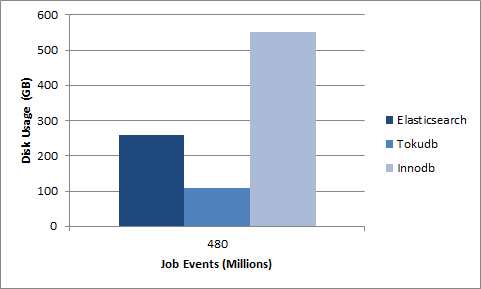
\includegraphics[scale=0.78]{figure/disksmall.png}
\caption{Disk usage after migrating data from CIMS instance with real data.}
\label{fig:disc}
\end{figure}

\begin{figure}[h!]
\centering
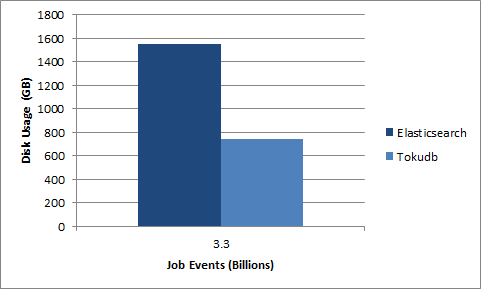
\includegraphics[scale=0.78]{figure/diskbig.png}
\caption{Disk usage after having a combination of real data and generated data.}
\label{fig:discbig}
\end{figure}

\subsection{Memory utilization}

\hiddensubsubsection{Elasticsearch}
In Elasticsearch some configuration related to memory usage is needed to achieve stable performance. It is recommended to set the JVM heap size that Elasticsearch uses to no more than half of total RAM available but never more than 32GB \cite{JVM, ESmemory}. Elasticsearch will typically use more memory than just the heap size, but this usage will be delegated to the operating system. Tests were done with 8GB, 16GB and 32GB heap size for both querying and insertion. Insertion using an 8GB heap would make Elasticsearch crash since garbage collection could not keep up. But 16 and 32GB gave stable insertion performance. However, there was no observable difference in insertion rates between 16 and 32GB heap sizes. Notably, when doing bulk insertion Elasticsearch would quickly reserve half of available system memory but no more (according to the default configuration). So insertion rates seem to scale with available RAM.

On the other hand querying was different. Performing many subsequent queries would not pool RAM like insertion did. Also no positive effect on response time could be observed by increasing the heap size. Elasticsearch was stable with 8, 16 and 32 heap sizes and response times were the same. 

\hiddensubsubsection{TokuDB}
The default configuration for TokuDB regarding memory utilization is the same as Elasticsearch, to use no more than half of total RAM available. During bulk insertion up to 3.3 billion rows using TokuDB, the database, similarly to Elasticsearch, quickly reserved half of available memory. No tweaking of the configuration was needed to get a stable system when doing bulk insertions. As such, the result is largely the same as for Elasticsearch; insertion rate again seem to scale with available RAM.


%\hiddensubsubsection{MongoDB}
%
%Working set estimations are presented in figure~\ref{fig:ws}. Initial estimations of the working set for MongoDB have been done with manual testing. As long as custom indexes defined on the job event collection fit in RAM, the database is stable and can respond to queries where indexes can be utilized. The working set estimation is the summed size of the custom indexes.
%
%\begin{figure}[h!]
%\centering
%\begin{tikzpicture}
%\begin{axis}[
%    ybar,
%    enlargelimits=0.15,
%    legend style={at={(0.5,-0.2)},
%      anchor=north,legend columns=-1, },
%    xlabel={Job Events (Billion)},
%    ylabel={Memory Utilization (GB)},
%    symbolic x coords={2,3.3},
%    xtick=data,
%    nodes near coords,
%    nodes near coords align={vertical},
%    ]
%\addplot coordinates {(2,6) (3.3,12)};
%\addplot coordinates {(2,1) (3.3,1)};
%\addplot coordinates {(2,1) (3.3,1)};
%\legend{MongoDB,ElasticSearch,MySQL}
%\end{axis}
%\end{tikzpicture}
%\caption{Working set estimation}
%\label{fig:ws}
%\end{figure}

\subsection{Insertion time}

\hiddensubsubsection{Elasticsearch}
Elasticsearch was configured to use a single node setup. The CIMS instance with 480 million job events was then migrated. With this configuration the process took 21 hours. This figure is not very reliable since it is also dependent on the database server of the CIMS instance. To get more dependable results we measured insertion rates for dummy data up to a total of 3.3 billion documents. The generation of data was performed locally. During the insertion of dummy data we could achieve a mean insertion rate of about 33 million documents per hour. This number, compared to the data generation rate in CIMS described in section~\ref{datagenrate} would mean that one month of data generated by a CIMS instance could be archived in less than a day. This is a positive result since it means that the archive system would spend little time doing insertions and most of its time responding the queries.

What is also notable is that even using a single node setup we observed little to no performance degradation for insert rates when the total data set grew. When generating documents from 0 to 3.3 billion the insert rate was as far as we could observe constant. In figure~\ref{fig:insert_rate}, we present a graph of insertion rates in relation to data set size.

\begin{figure}[h!]
\centering
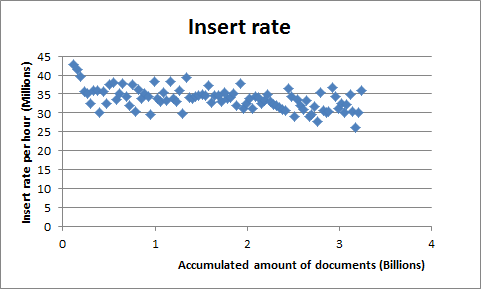
\includegraphics[]{figure/insert_rate.png}
\caption{Insertion rate of dummy job event data into Elasticsearch.}
\label{fig:insert_rate}
\end{figure}

When switching to a cluster with 4 nodes (4 Elasticsearch instances running on the same machine), much greater insert rates could be achieved and we observed an initial insert rate of 60 million documents per hour in this case.

These reported insertion rates were achieved with little configuration of Elasticsearch. The only important configuration variable to set is the JVM heap size, which as previously mentioned was set to a minimum of 16GB to get stable performance.

The insertion rate measurements show that Elasticsearch is more than capable of handling the current growth trends.

%\hiddensubsubsection{MongoDB}

\hiddensubsubsection{TokuDB}
A MySQL instance using TokuDB was setup using mostly standard default options. Insertion of dummy data was then performed in the same way as with Elasticsearch. In figure~\ref{fig:insert_rate_tokudb} a graph with insertion rates is shown. In this case some degradation seems to exist over time. However, considering the current growth trends, these insertion rates are still much higher than the amount of data that gets generated by a CIMS instance. Therefore the insertion rates should still be considered acceptable.
\begin{figure}[h!]
\centering
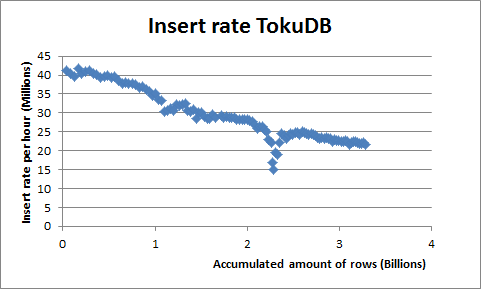
\includegraphics[]{figure/insert_rate_tokudb.png}
\caption{Insertion rate of dummy job event data into MySQL/TokuDB.}
\label{fig:insert_rate_tokudb}
\end{figure}

\subsection{Query response time}
Measurements were made in regards to query response time with the large data set (3.3 billion documents) containing dummy job events. We looked specifically at two queries in this case, namely to look up a job event by its name (used for creating test case histories) and to look up all children for a job event (used to create a test tree). For the former query, the result set will grow as the overall data set grows, since more and more test cases with a specific name is inserted. Another interesting thing to note about this query is that data retrieval is random across the data set since test cases with the same name exist in many builds spanning years' of time.

For the latter, the result set size will likely grow much more slowly. It is not dependent on the overall data set size but instead depends on if the size of test suites grow. This is in the hands of the developers who construct the test suites. In comparison to looking up a test case by name, looking up test suite children is not random across the entire data set. This because test cases from the same build and test suite are inserted together. As such, querying for test suite children should be faster than querying by test case name. But the response time is also highly dependent on the size of the result set.

As stated previously, the purpose of these tests is not to prove or make claims about which solution is better but rather to assess if they perform adequately. It is likely that there is room for improvement in our configuration and code that would give even better results. 

\hiddensubsubsection{Elasticsearch}
In figure~\ref{fig:query_by_name} the response times when querying by name is shown. The figure has 400 data points in total, where for each point a name is selected randomly from a list of all names of test cases from one CIMS instance. There are about 16000 unique names in total. The outliers in the figure are due to that a name was selected more than once and results where cached for the second the time query was executed with the same name. Notably, the response time is long for this query because of the large result sets. If the whole result set is not needed but only the first few hundred hits, a more realistic scenario in every day usage, then the response time would reduce to a few seconds.

The second chosen query, to look up all the children of a test suite was tested on the large data set and provided promising results. In the large data set, the dummy data that was generated have test suites all containing 1000 children test cases. In the test that was performed, the average response time when querying for all children of a test case was 0.134 seconds.

\begin{figure}[h!]
\centering
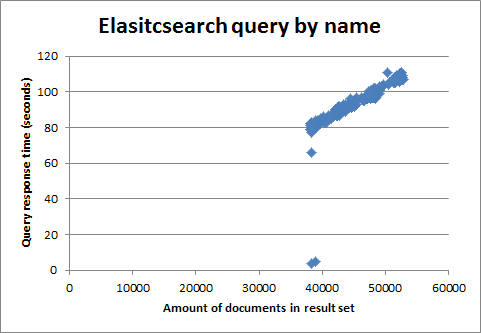
\includegraphics[]{figure/es_by_name.png}
\caption{Query response time in Elasticsearch when looking up job events by name.}
\label{fig:query_by_name}
\end{figure}

\hiddensubsubsection{TokuDB}
Figure~\ref{fig:toku_by_name} shows response time for TokuDB when querying by name. 400 test case names were selected randomly and subsequently queried on. We note that, when querying by name, TokuDB is slower overall than Elasticsearch but that the response times are still very reasonable, given the size of the result sets. As for Elasticsearch, subsequent queries on the same name means results are cached and thus finish in just a few seconds. 
Querying for all children of a test suite showed good results for TokuDB where the average response time was 0.102 seconds for test suites with 1000 children test cases.

\begin{figure}[h!]
\centering
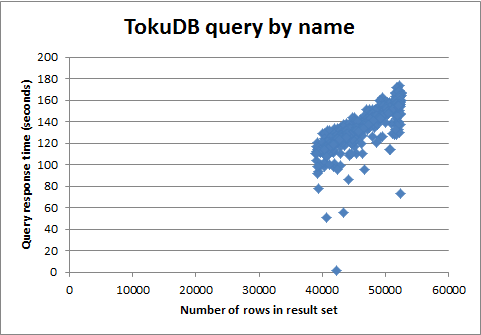
\includegraphics[]{figure/toku_by_name.png}
\caption{Query response time in MySQL/TokuDB when looking up job events by name.}
\label{fig:toku_by_name}
\end{figure}
%Get job event ny name \\
%asddfgsdf, 90 seconds, 60k events \\
%alsjkd, 90 seconds, 60k events \\
%askdlj, 90 seconds, 60k events \\
%aslkdjasd, 90 seconds, 60k events \\
%oipioipi, 90 seconds, 60k events \\
%iyuiytyuie, 90 seconds, 60k events \\
%
%Get job event children \\
%2394234-290384, 5 seconds, 1k events \\
%2394234-290384, 5 seconds, 1k events \\
%2394234-290384, 5 seconds, 1k events \\
%2394234-290384, 5 seconds, 1k events \\
%2394234-290384, 5 seconds, 1k events \\
%2394234-290384, 5 seconds, 1k events \\

\section{Schema changes}
Given that one of the main problems with the current implementation of CIMS is long running schema migrations in MySQL using InnoDB, an archive prototype must effectively address this issue and minimize or remove the need to perform these schema migrations.

\hiddensubsection{Elasticsearch}
Elasticsearch has the data model of a document-store in that it stores data in the JSON format and does not enforce a predefined schema on inserted documents. This means that the need to perform schema migrations is basically removed and that data with varying structure can be inserted. As already mentioned, this was one of the main reasons for choosing a document-store as a candidate for the archive database.

\hiddensubsection{TokuDB}
When using a relational database as an archive database, the schema between the live database and the archive needs to be kept in sync. TokuDB has basically solved the issue of long running schema migrations by introducing concepts like hot schema changes and lazy migration. When performing an alter table operation on a table, the change is not immediately propagated to disc for all rows, instead it is done the next time the row is retrieved by a query like a select statement. As such, typical alter tables operations using TokuDB reduces to a few seconds, even on huge tables.

Performing schema changes was tested on the large data set with 3.3 billion rows with good results. For example, adding a new integer column with a default value to the job event table took just a few seconds.

\subsection{Horizontal Scalability}
While Elasticsearch performed well in tests using a single node setup with large data sets, having the possibility to go smoothly from single node to cluster is important to consider. Before adding more nodes to an Elasticsearch cluster, the amount of shards per index must be defined as it sets the upper bound for the total amount possible nodes in the cluster.

In Elasticsearch, all data in an index is split up into shards. These shards can themselves not be split and as such, one shard is always stored in its entirety on a single node. However, nodes can store multiple shards from the same index, as is the case in the single node setup that was tested on. In this setup, four total shards were predefined per index. In production, the total number of shards is typically set to a much higher amount. 

Given the setup that was predefined, the maximum number of deployable nodes was four. The single node setup was then converted to a four node cluster where all nodes resided on the testing machine. Doing the conversion was as trivial as starting new Elasticsearch processes configured with the same cluster name an already running Elasticsearch process. The cluster then automatically handles shard allocation to available nodes.

%Not yet addressed
%Här borde vi kunna skriva tekniska saker, men från de tekniska saker dra slutsater i Discussion som svarar på om dessa tekniker ger något business value?
%%\hiddensubsubsection{MongoDB}
%\hiddensubsubsection{Elasticsearch}
%"Lessons learned while scaling with Elasticsearch, future work can be to test with more nodes".\\
%Compared to MongoDB, horizontal scaling with Elasticsearch demands more configuration upfront in order to get a suitable cluster.
%In MongoDB, an arbitrary number of nodes can be added to the cluster. The maximum number of nodes in an Elasticsearch cluster can never be higher then the total amount of shards, which must be defined when an index (collection of documents) is created.
%
%%This restriction depends on how Elasticsearch is scaling in an horizontal manner. The partitioning of data when adding new nodes to a cluster is dependent on how many shards the initial node holds, as an new node is added to the cluster it overtakes shards from the already existing nodes.
%
%\hiddensubsubsection{TokuDB}

\section{Integration with CIMS}
Proof of concept functionality was requested by stakeholders at Ericsson to demonstrate the possibility of integrating the archive with CIMS and the suitability of polyglot persistence. As mentioned previously, the viewing of builds was selected as a suitable piece of functionality to evolve to use the archive. 

To demonstrate the new archive build viewer we used the following somewhat contrived use case as a basis;
\begin{itemize}
\item Initially the archive is empty.
\item User views list of all builds.
\item User identifies build that has a reference build.
\item User deletes the reference build.
\item System moves build to archive before it is deleted.
\item User requests to view reference build.
\item System presents data about reference build using the archive API.
\end{itemize}

This use case is mostly used for demonstration purposes and we believe a more realistic way of moving data from the live database to the archive would be to use scheduled jobs that do this on for example a weekly basis.

It was possible with reasonable effort to implement the new build viewer in CIMS and use the archive API to present build data. However, the view was somewhat simplified given time constraints and because of the way CIMS is designed, where it is not trivial to change the underlying data source for web page components. Overall, through this implementation it is shown that to be possible without too much effort to integrate the archive with CIMS.

%Initially the archive contains no data. A user views the list of all builds and finds a build that has a reference build. The user then goes on to delete the reference build. Before the build is deleted from the relational database it is first migrated to the archive. Then when requesting to view the reference build, the archive will be used to present it instead of the relational database. On this new build page it can be noted that it is the archive that is used as the underlying data source and the page also contains links to view the raw build and test data in Elasticsearch.


\section{Organizational suitability}
This chapter ends with discussion about what was found out about the organizational suitability of the two constructed prototypes.

%\hiddensubsection{MongoDB}

\hiddensubsection{Elasticsearch}
There are a few reasons as to why we believe using Elasticsearch would work well for the organization. First of all, CIMS already employs a number of different\footnotemark\ data stores other than MySQL, so in some sense it is already a polyglot persistence solution. Therefore, development of CIMS requires familiarity with multiple databases and their respective ways of representing data. Going from this situation to also using Elasticsearch should not be considered too problematic. Through discussion with the CIMS development team this opinion is somewhat cemented as they are very open to discussing and trying out new technologies and have been doing so before this thesis was conducted. 

\footnotetext{CIMS uses Redis \cite{redis} and Sphinx \cite{sphinx} for caching.}

Furthermore, in an article by Stonebraker and Cattell \cite{10rules}, several rules are given to aid the selection of what they classify as simple operation data stores, namely databases that scale horizontally and avoid complex operations like cross node joins. One notable rule is to consider out-of-the-box behavior of a candidate database. The better this behavior is the less of a pain it will be to initially configure the candidate database. We, the authors of this thesis, do not make any claim to be database experts but our experience of Elasticsearch and its out-of-the-box behavior is certainly positive in many respects. The amount of configuration to get stable performance was minimal. As mentioned earlier, the only variable we had to consider in order to get stable performance was the JVM heap size. On top of this, it was easy to go from a single node setup to a cluster. 

However, while the initial configuration was pain free, there are many things to consider when it comes to schema and query design in Elasticsearch. For example, it is important to know upfront what kinds of queries that the field of a document or the document as a whole should support. Notably, if a field requires to be queried on by an exact value comparison, this must be configured upfront (typically by declaring the field as 'not analyzed'). As such, most of the time spent on Elasticsearch was not done configuring the database but rather optimizing schemas and exploring the rich query possibilities.

Overall, we think Elasticsearch is an interesting candidate to consider moving forward and see no real problems as to why it would not be possible to use, taking the organizational context into consideration.

\hiddensubsection{TokuDB}
Since TokuDB is a storage engine for MySQL, for this solution the live database and the archive would be identical for everything but the storage engine. As such, this solution has very little friction to use as everyone working with CIMS is already very knowledgeable about relational databases and MySQL in particular. The solution is simple and would solve many of identified problems related to monotonic data growth. Through the other points of evaluation for TokuDB we have shown that by using TokuDB as a storage engine, it is very possible to scale to billions of rows on a single machine when it comes to both insertion rate and query performance.